\documentclass[aspectratio=169]{beamer}

\usetheme{default}

\usepackage[utf8]{inputenc}
\usepackage[russian]{babel}
\usepackage[OT1]{fontenc}
\usepackage{amsmath}
\usepackage{amsfonts}
\usepackage{amssymb}
\usepackage{graphicx}
\usepackage{etoolbox}
\usepackage{caption}
\usepackage{subcaption}
\captionsetup{compatibility=false}
\usepackage{pifont}
%\usepackage{subfigure}
\usepackage{xcolor}
\usepackage{framed}
\usepackage{empheq}
\usepackage[many]{tcolorbox}
\usepackage{multirow}
\usepackage{tikz}
\usepackage{listings}
\usepackage{tikz}

\definecolor{shadecolor}{cmyk}{0,0,0,1}

\lstset{
	backgroundcolor=\color{lightgray},
	commentstyle=\color{blue},
	frame=single
	breakatwhitespace, 
	language=python, 
	columns=fullflexible, 
	keepspaces, 
	breaklines, 
	tabsize=3, 
	showstringspaces=false, 
	extendedchars=true,
	numbers=left
}

\makeatletter

\setbeamercolor{title}{fg=white}
\setbeamercolor{frametitle}{fg=black}
\setbeamerfont*{title}{family=\sffamily,size=\LARGE}

\setbeamerfont{page number in head/foot}{size=\scriptsize}
\setbeamertemplate{footline}[frame number]
\let\otp\titlepage
\renewcommand{\titlepage}{\otp\addtocounter{framenumber}{-1}}

\setbeamertemplate{background canvas}{%
	\ifnumequal{\c@framenumber}{0}{%
		\vbox to \paperheight{\vfil\hbox to \paperwidth{\hfil
\includegraphics[height=\paperheight]{images/cover.png}\hfil}\vfil}
   }{%
      \ifnumequal{\c@framenumber}{\inserttotalframenumber}{
        \vbox to \paperheight{\vfil\hbox to \paperwidth{\hfil
\includegraphics[height=\paperheight]{images/back.png}\hfil}\vfil}
      }{%
         % Other frames
      }%
   }%
}

\makeatother

\beamertemplatenavigationsymbolsempty

\tcbset{highlight math style={enhanced,colframe=red,colback=white,arc=4pt,boxrule=1pt}}

\usetikzlibrary{shadings,shadows,shapes.arrows}

\newcommand*{\tikzarrow}[2]{%
  \tikz[
    baseline=(A.base),             % Set baseline to the baseline of node content
    font=\footnotesize\sffamily    % Set fontsize of the node content
  ]
  \node[
    single arrow,                  % Shape of the node
    single arrow head extend=5pt,  % Actual width of arrow head
    draw,                          % Draw the node shape
    inner sep=3pt,                 % Separation between node content and node shape
    top color=#1,               % Shading color on top of node
    bottom color=#1,               % Shading color on bottom of node
    % drop shadow                    % Draw a shadow
  ] (A) {#2};%
}

\newcommand{\tikzfancyarrow}[2][2cm]{\tikz[baseline=-0.5ex]\node [arrowstyle=#1] {#2};}
\newcommand*\rot{\rotatebox{90}}

\author{Николай Анохин}
\title{\newline \newline \newline Лекция 6 \\ Классификация текстов и Naive Bayes}

\begin{document}

\begin{frame}[plain]
\titlepage
\end{frame}

\begin{frame}{План занятия}
\tableofcontents
\end{frame}

% ============================================== %

\section{Обработка текстов}

% ============================================== %

\begin{frame}{}

\begin{center}
\Large Обработка текстов

\vspace{1em}
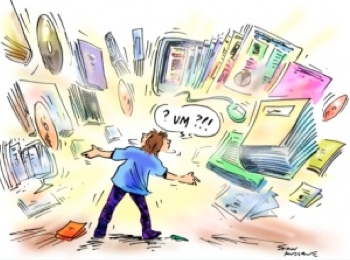
\includegraphics[height=0.5\textheight]{images/text.png}
\end{center}

\end{frame}

\begin{frame}{Data Mining vs Text Mining}

	\begin{columns}[T]
    \begin{column}{.5\textwidth}
   	Data Mining: \\ извлечение {\it неочевидной} информации

	\vspace{1em}
	Text Mining: \\ извлечение {\it очевидной} информации

\vspace{1em}
Трудности
\begin{itemize}
\item Огромные объемы
\item Отстутсвие структуры
\end{itemize}
	    
    \end{column}
    \begin{column}{.5\textwidth}
    \vspace{1em}
    
\includegraphics[scale=0.06]{images/books.jpg}    
    \end{column}
  \end{columns}

\end{frame}

% ============================================== %

\begin{frame}{Задачи Text Mining}

\begin{itemize}
\item Суммаризация текста \\
{\it агрегация новостей}
% Nick D'Aloisio 30M in 2013
\item Классификация и кластеризация документов \\
{\it категоризация, антиспам, sentiment analysis, opinion mining}
% Кинопоиск
\item Извлечение метаданных \\
{\it определение языка, автора, тегирование}
% Автор постов на форуме
\item Выделение сущностей \\
{\it места, люди, компании, почтовые адреса}
% Определение сущностей для ссылок Википедию
\end{itemize}

\end{frame}

% ============================================== %

\begin{frame}{Этапы (простой) обработки текста}

\begin{center}
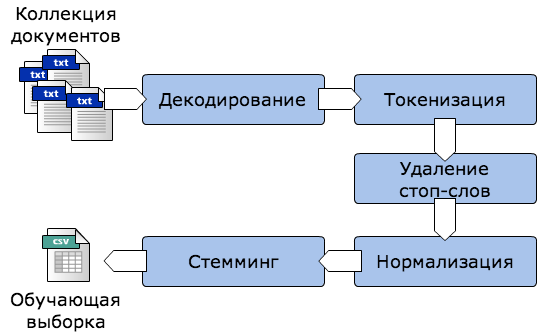
\includegraphics[scale=0.5]{images/textm.png}
\end{center}

\end{frame}

% ============================================== %

\begin{frame}{Декодирование}

\begin{block}{Def.}
перевод последовательности байт в последовательность символов
\end{block}

\begin{itemize}
\item Распаковка \\
{\it plain/.zip/.gz/...}
\item Кодировка \\
{\it ASCII/utf-8/Windows-1251/...}
\item Формат \\
{\it csv/xml/json/doc...}
\end{itemize}

Кроме того: что такое документ?

\end{frame}

% ============================================== %

\begin{frame}{Разбиение на токены}

\begin{block}{Def.}
разбиение последовательности символов на части (токены), возможно, исключая из рассмотрения некоторые символы
\end{block}

\vspace{1em}
{\it Наивный подход:} разделить строку пробелами и выкинуть знаки препинания
\begin{quote}
Трисия любила {\bf Нью-Йорк}, поскольку любовь к Нью-Йорку могла положительно повлиять на ее карьеру.
\end{quote}

{\it Проблемы:}
\begin{itemize}
\item n.anokhin@corp.mail.ru, 127.0.0.1
\item С++, C\#
\item {\it York University} vs {\it New York University}
\item Зависимость от языка (``Lebensversicherungsgesellschaftsangestellter'', ``l'amour'')
\end{itemize}

{\it Альтернатива:} n-граммы

\end{frame}

% ============================================== %

\begin{frame}[fragile]{Разбиение на токены}

\begin{shaded}
{\color{green}
\begin{verbatim}
>>> from nltk.tokenize import RegexpTokenizer
>>> tokenizer = RegexpTokenizer('\w+|[^\w\s]+')
>>> s = u'Трисия любила Нью-Йорк, поскольку любовь \
... к Нью-Йорку могла положительно повлиять на ее карьеру.'
>>> for t in tokenizer.tokenize(s)[:7]: print t + " ::",
... 
Трисия :: любила :: Нью :: - :: Йорк :: , :: поскольку ::
\end{verbatim}
}
\end{shaded}

\end{frame}

% ============================================== %

\begin{frame}[fragile]{Стоп-слова}

\begin{block}{Def.}
Наиболее частые слова в языке, не содержащие никакой информации о содержании текста
\end{block}

\begin{shaded}
{\color{green}
\begin{verbatim}
>>> from nltk.corpus import stopwords
>>> for sw in stopwords.words('russian')[1:20]: print sw,
... 
в во не что он на я с со как а то все она так его но да ты
\end{verbatim}
}
\end{shaded}

\vspace{1em}
Проблема: ``To be or not to be"

\end{frame}

% ============================================== %

\begin{frame}[fragile]{Нормализация}

\begin{block}{Def.}
Приведение токенов к единому виду для того, чтобы избавиться от поверхностной разницы в написании
\end{block}

\vspace{1em}
Подходы
\begin{itemize}
\item сформулировать набор правил, по которым преобразуется токен
\begin{quote}
Нью-Йорк $\rightarrow$ нью-йорк $\rightarrow$ ньюйорк $\rightarrow$ ньюиорк
\end{quote}
\item явно хранить связи между токенами (\href{http://wordnetweb.princeton.edu/perl/webwn}{WordNet} -- Princeton)
\begin{quote}
машина $\rightarrow$ автомобиль, Windows $\not \rightarrow$ window
\end{quote}
\end{itemize}

\end{frame}

% ============================================== %

\begin{frame}[fragile]{Нормализация}

\begin{shaded}

{\color{green}
\begin{verbatim}
>>> s = u'Нью-Йорк'
>>> s1 = s.lower()
>>> print s1
нью-йорк
>>> s2 = re.sub(ur"\W", "", s1, flags=re.U)
>>> print s2
ньюйорк
>>> s3 = re.sub(ur"й", u"и", s2, flags=re.U)
>>> print s3
ньюиорк
\end{verbatim}
}
\end{shaded}

\end{frame}

% ============================================== %

\begin{frame}{Стемминг и Лемматизация}

\begin{block}{Def.}
Приведение грамматических форм слова и однокоренных слов к единой основе (lemma): 
\begin{itemize}
\item Stemming -- с помощью простых эвристических правил
\begin{itemize}
\item Porter (Cambridge -- 1980) \\
5 этапов, на каждом применяется набор правил, таких как
\[
sses \rightarrow ss \quad (\text{caresses}\rightarrow\text{caress})
\]
\[
ies \rightarrow i \quad (\text{ponies}\rightarrow\text{poni})
\]
\item Lovins (1968)
\item Paice (1990)
\item еще 100500
\end{itemize}
\item Lemmatization -- с использованием словарей и морфологического анализа
\end{itemize}
\end{block}

\end{frame}

% ============================================== %

\begin{frame}[fragile]{Стемминг}

\begin{shaded}
{\color{green}
\begin{verbatim}
>>> from nltk.stem.snowball import PorterStemmer
>>> s = PorterStemmer()
>>> print s.stem('tokenization'); print s.stem('stemming')
token
stem
>>> from nltk.stem.snowball import RussianStemmer
>>> r = RussianStemmer()
>>> print r.stem(u'Авиация'); print r.stem(u'национальный')
авиац
национальн
\end{verbatim}
}
\end{shaded}

\begin{block}{Наблюдение}
для сложных языков лучше подходит лемматизация
\end{block}

\end{frame}

% ============================================== %

\begin{frame}{Heap's law}

\[
M = k T^\beta, \;M \text{ -- размер словаря}, \; T \text{ -- количество слов в корпусе}
\]
\[
30 \leq k \leq 100, \; b \approx 0.5
\]


\begin{center}
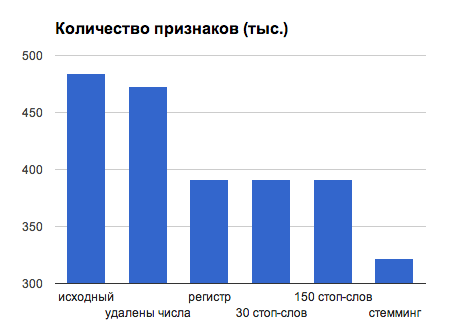
\includegraphics[scale=0.35]{images/dim.png}\;
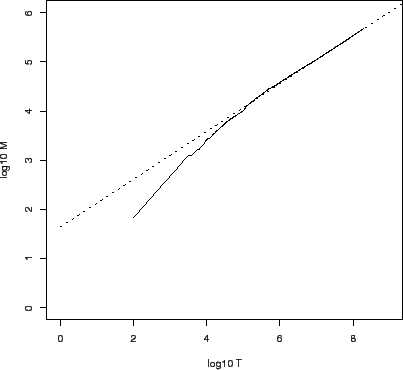
\includegraphics[scale=0.3]{images/heaps.png}
\end{center}

\end{frame}

% ============================================== %

\begin{frame}{Представление документов}

{\bf Boolean Model.} Присутствие или отсутствие слова в документе

\vspace{1em}
{\bf Bag of Words.} Порядок токенов не важен
\begin{quote}
Погода была ужасная, принцесса была прекрасная. \\ Или все было наоборот?
\end{quote}

Координаты
\begin{itemize}
\item Мультиномиальные: количество токенов в документе
\item Числовые: взвешенное количество токенов в документе
\end{itemize}

\end{frame}

% ============================================== %

\begin{frame}{Zipf's law}

\begin{columns}[T]
    \begin{column}{.5\textwidth}
   	$t_1, \ldots, t_N$ -- токены, отранжированные по убыванию частоты
   	
	$f_1, \dots, f_N$ -- соответствующие частоты

	\vspace{1em}
	\begin{framed}
	{\bf Закон Ципфа}
	\[
	f_i = \frac{c}{i^k}
	\]	
	\end{framed}
	
	Что еще? Посещаемость сайтов, количество друзей, население городов...
	    
    \end{column}
    \begin{column}{.5\textwidth}
    \vspace{1em}
    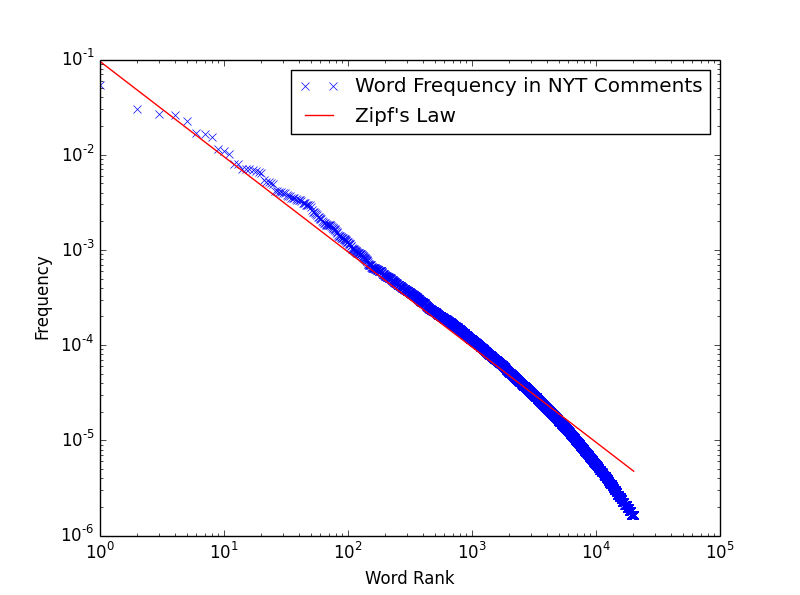
\includegraphics[scale=0.3]{images/zipf.png}    
    \end{column}
  \end{columns}

\end{frame}

% ============================================== %

\begin{frame}{Задача}

Дана коллекция, содержащая $10^6$ (не уникальных) токенов. Предполагая, что частоты слов распределены по закону
\[
f_i = \frac{c}{(i + 10)^2},
\]
оцените
\begin{itemize}
\item количество вхождений наиболее часто встречающегося слова
\item количество слов, котоые встречаются минимум дважды
\end{itemize}

\vspace{1em}
{\it Подсказка: $\sum_{i=11}^{\infty}\frac{1}{i^2} \approx 0.095$}

\end{frame}

% ============================================== %

\begin{frame}{BoW \& TF-IDF}

\vspace{1em}
Количество вхождений слова $t$ в документе $d$
\[
TF_{t,d} = term\!\!-\!\!frequency(t, d)
\]
Количество документов из $N$ возможных, где встречается $t$
\[
DF_t = document\!\!-\!\!fequency(t)
\]
\[
IDF_t = inverse\!\!-\!\!document\!\!-\!\!frequency(t) = \log \frac{N}{DF_t}
\]
TF-IDF
\[
TF\!\!-\!\!IDF_{t,d} = TF_{t,d} \times IDF_t
\]

\end{frame}

% ============================================== %

\section{Naive Bayes}

% ============================================== %

\begin{frame}{}

\begin{center}
\Large Naive Bayes

\vspace{1em}
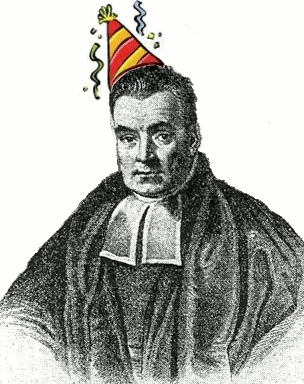
\includegraphics[height=0.6\textheight]{images/bayes.png}
\end{center}

\end{frame}

\begin{frame}{Байесовский классификатор}

Дано

$\mathbf{x} \in X$ -- описание документа $d$ из коллекции $D$ \\
$C_k \in C, \; k = 1,\ldots,K$ -- целевая переменная

\vspace{1em}
Теорема Байеса
\[
P(C_k \mid \mathbf{x}) = \frac{p(\mathbf{x} \mid C_k) p(C_k)}{p(\mathbf{x})} \propto p(\mathbf{x} \mid C_k) p(C_k)
\]
Принцип Maximum A-Posteriori
\[
C_{MAP} = \arg \max_k p(C_k | \mathbf{x})
\]

\end{frame}

% ============================================== %

\begin{frame}{Naive Bayes}

$x_j$ -- слово на $j$-м месте в документе $\mathbf{x}$,
$w^i \in V$ -- слово из словаря $V$

\vspace{1em}
Предположения
\begin{enumerate}
\item conditional independence 
\[
p(x_i=w^s, x_j=w^r | C_k) = p(x_i=w^s | C_k) p(x_j=w^r | C_k)
\]
\item positional independence
\[
P(x_i=w^s | C_k) = P(x_j=w^s | C_k) = P(x = w^s | C_k)
\]
\end{enumerate}

Получаем
\[
p(\mathbf{x} | C_k) = p(x_1=w^{s_1}, \ldots, x_{|\mathbf{x}|}=w^{s_{|\mathbf{x}|}} | C_k) = \prod_{i=1}^{|\mathbf{x}|} p(x = w^{s_i} | C_k)
\]

\begin{block}{Почему NB хорошо работает?}
Корректная оценка дает правильное предсказание, но правильное предсказание {\it не требует} корректной оценки
\end{block}

\end{frame}

% ============================================== %

\begin{frame}{Варианты NB}

MAP
\[
C_{MAP} = \arg \max_k \prod_{i=1}^{|\mathbf{x}|} p(x = w^{s_i} | C_k) p(C_k) = 
\]
\[
= \arg \max_k \left[ \log p(C_k) + \sum_{i=1}^{|\mathbf{x}|} \log p(x = w^{s_i} | C_k) \right]
\]
Априорные вероятности
\[
p(C_k) = N_{C_k}/{N}
\]
Likelihood $p(x = w^{s_i} | C_k)$
\begin{itemize}
\item BernoulliNB $p(x = w^{s_i} | C_k) = D_{w^{s_i}, C_k} / D_{C_k}$, $D$ -- кол-во документов
\item MultinomialNB $p(x = w^{s_i} | C_k) = T_{w^{s_i}, C_k} / T_{C_k}$, $T$ -- кол-во токенов
\item GaussianNB $p(x = w^{s_i} | C_k) = \mathcal{N}(\mu_k, \sigma_k^2)$, параметры из MLE
\end{itemize}

\end{frame}

% ============================================== %

\defverbatim[colored]\nbtrain{%
\begin{lstlisting}[tabsize=4,basicstyle=\ttfamily]
function nb_train(D,C):
	V = dictionary of tokens
	N = number of documents
	for Ck in C: # iterate over all classes
		N_Ck = number of documents in class Ck
		p(Ck) = N_Ck / N # Class prior
		D_Ck = Documents in class Ck		
		for w_i in V:			
			# multinomial, bernoulli, gaussian
			p(w_i|Ck) = count_likelihood(...)
	return V, p(Ck), p(w_i|Ck)
\end{lstlisting}
}

\begin{frame}{Обучение NB}

\nbtrain

\vspace{1em}
Алгоритмическая сложность: $O(|D| \langle |\mathbf{x}| \rangle + |C||V|)$

\end{frame}

% ============================================== %

\defverbatim[colored]\nbapply{%
\begin{lstlisting}[tabsize=4,basicstyle=\ttfamily]
function nb_apply(d, C, V, p(Ck), p(w_i|Ck)):
	x = tokenize(d) # somehow	
	for Ck in C: # iterate over all classes
		score(Ck|x) = log p(Ck) # use class prior
		# use likelihoods
		for i in 1..|x|:		
			score(Ck|x) += log p(x_i|Ck)
	return arg max score(Ck|x)
\end{lstlisting}
}

\begin{frame}{Применение MultinomialNB}

\nbapply

\vspace{1em}
Алгоритмическая сложность: $O(|C||\mathbf{x}|)$

\end{frame}

% ============================================== %

\begin{frame}{Задача}

\begin{tabular}{l p{7cm} r}
d & Текст & Класс \\
\hline
1 & котики такие мокрые & мимими \\
2 & пушистые котики няшки & мимими \\
3 & морские котики  & не мимими \\
4 & мокрые морские свинки & не мимими \\
\hline
5 & котики мокрые & ???
\end{tabular}

\vspace{1em}
С помощью алгоритма MultinomialNB вычислить $p(\text{мимими} | d_5)$

\end{frame}

% ============================================== %

\begin{frame}{Сглаживание}

{\bf Проблема:} $p(\text{свинки}|\text{мимими}) = 0$

\vspace{1em}
{\bf Решение:}
\[
p(x = w_{s_i} | C_k) = \frac{T_{w_{s_i}, C_k} + \alpha}{T_{C_k} + \alpha |V|}
\]
если $\alpha \geq 1$ -- сглаживание Лапласа, если $0 \leq \alpha \leq 1$ -- Лидстоуна

\vspace{1em}
\begin{exampleblock}{Упражнение}
С учетом сглаживания вычислить 
\[
p(\text{пушистые}|\text{не мимими}), \; p(\text{пушистые}|\text{мимими}).
\]
\end{exampleblock}

\end{frame}

% ============================================== %

\begin{frame}{Генеративная модель}

\begin{center}
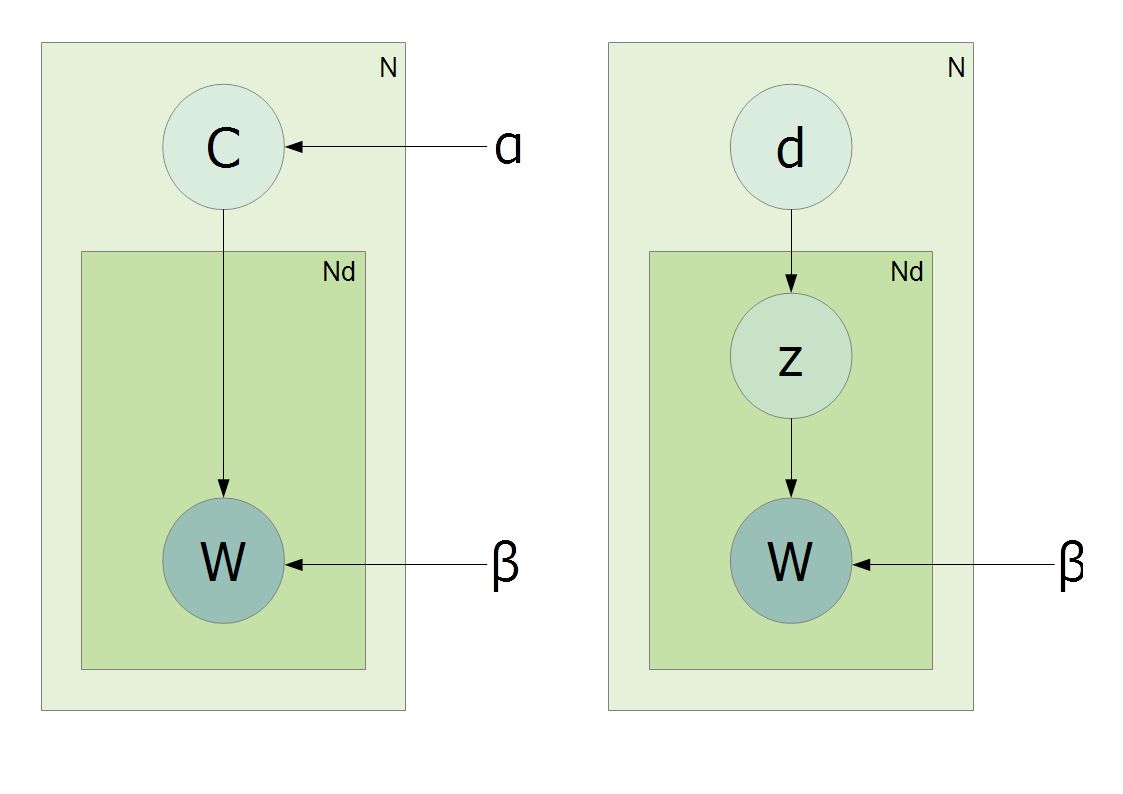
\includegraphics[scale=0.3]{images/lsa.png}
\end{center}

\end{frame}

% ============================================== %

\begin{frame}{Байесовские сети}

\begin{center}
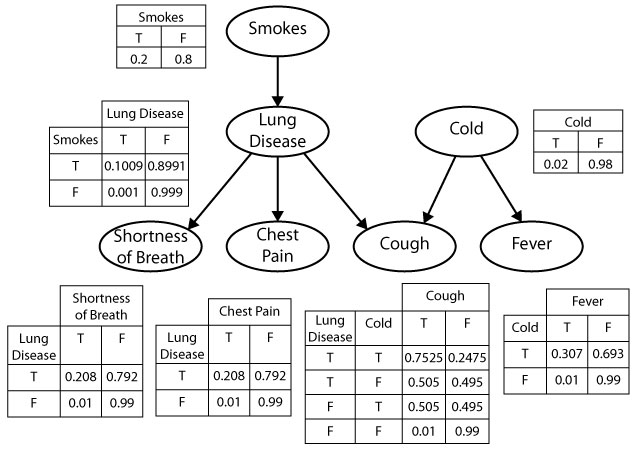
\includegraphics[scale=0.4]{images/network.jpg}
\end{center}

\end{frame}

% ============================================== %

\begin{frame}{Итоги}

\begin{itemize}
\item[+] Генеративная модель
\item[+] (Удивительно) неплохо работает
\item[+] Стабилен при смещении выборки (aka concept drift)
\item[+] Оптимальный по производительности
\end{itemize}

\begin{itemize}
\item[--] Наивные предположения
\item[--] Требует отбора признаков
\end{itemize}

\end{frame}

% ============================================== %

\begin{frame}{}

\begin{center}
\Large Вопросы
\end{center}

\end{frame}

\end{document}